\documentclass[pra,12pt]{revtex4}
\usepackage{amsmath}
\usepackage{amssymb}
\usepackage{graphicx}
\usepackage{color}
\usepackage{framed}
\usepackage[pdfborder={0 0 0},colorlinks=true,linkcolor=blue,urlcolor=blue]{hyperref}

\def\ket#1{\left|#1\right\rangle}
\def\bra#1{\left\langle#1\right|}
\def\braket#1{\left\langle#1\right\rangle}

\usepackage{fancyhdr}
\fancyhf{}
\lhead{\tiny Y.~D.~Chong}
\rhead{\scriptsize PH4401: Quantum Mechanics III}
\lfoot{}
\rfoot{\thepage}
\pagestyle{fancy}

\setlength{\parindent}{14pt}
\renewcommand{\theequation}{C.\arabic{equation}}
\renewcommand{\thesection}{C\arabic{section}}

\renewcommand{\baselinestretch}{1.0}
\setlength{\parskip}{0.07in}

\begin{document}

\begin{center}
{\large \textbf{Appendix C: Entropy}}
\end{center}

``Entropy'' is an important theoretical concept that provides a way to
quantify one's lack of knowledge about a complex system.  It is used
in multiple fields of science and mathematics; in thermodynamics and
statistical mechanics, \textbf{thermodynamic entropy} describes the
uncertainty about the precise microscopic details, or ``microstate'',
of a large physical system.  In information theory, the quantity
called \textbf{information entropy}, also called \textbf{Shannon
  entropy} after its inventor Claude Shannon, describes the
uncertainty about the contents of a transmitted message.  One of the
most profound developments in theoretical physics in the 20th century
was the discovery by E.~T.~Jaynes that statistical mechanics can be
formulated in terms of information theory; hence, the
thermodynamics-based and information-based concepts of entropy are one
and the same.  For details about this topic, see
\hyperref[cite:jaynes]{Jaynes (1957)} and
\hyperref[cite:jaynes2]{Jaynes (1957a)}.  In this appendix, we will
summarize the definition of entropy in classical physics, and how it
is related to other physical quantities.

\section{Definition}
\label{sec:entrodef}

Suppose a system has $W$ discrete microstates labeled by integers
$\{1,2,3,\dots, W\}$ , which have probabilities $\{p_1, p_2, p_3,
\dots, p_W\}$.  Then the entropy of the system is defined as
\begin{equation}
  S = - k_b \, \sum_{i=1}^W p_i \ln(p_i),
  \label{Sdef}
\end{equation}
where $k_b$ is Boltzmann's constant.  The probabilities $p_i$ are
\textit{conditional} probabilities, conditioned on the set of known
macroscopic features of the system.  For example, if we know the
system's total energy, the set of microstates used in Eq.~\eqref{Sdef}
can only include microstates which have precisely that energy.

Consider the behavior of $S$ under two extreme scenarios:

\begin{itemize}
\item Suppose the microstate is completely certain, i.e., $p_k = 1$
  for some $k$.  Then $S = 0$.

\item Suppose there are $W$ possible microstates, each with equal
  probabilities
  \begin{equation}
    p_i = \frac{1}{W} \;\;\forall i \in \{1,2,\dots,W\}.
  \end{equation}
  This describes a scenario of complete uncertainty between the
  possible choices.  Then
  \begin{equation}
    S \,=\, -k_b W \frac{1}{W} \ln(1/W) \;=\; k_b \ln W.
  \end{equation}
\end{itemize}

\noindent
The entropy formula is designed so that any other probability
distribution, which refers to a situation of \textit{partial}
uncertainty, yields an entropy $S$ lying between $0$
and $k_b \ln W$.

\pagebreak

\section{Upper and lower bounds}

To see that zero is the lower bound for the entropy, note that for $0
\le p_i \le 1$, each term in the entropy formula \eqref{Sdef}
satisfies $-k_b\, p_i\ln(p_i) \ge 0$, and the equality holds if and
only if $p_i = 0$ or $p_i = 1$.  This is illustrated in the figure
below:

\begin{figure}[h!]
  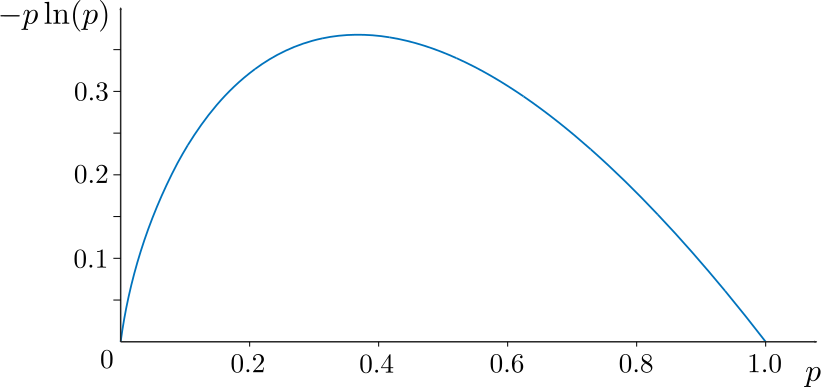
\includegraphics[width=0.55\textwidth]{plogp}
\end{figure}

\noindent
This implies that $S\ge 0$.  Moreover, $S = 0$ if and only if $p_i =
\delta_{ik}$ for some $k$ (i.e., there is no uncertainty about which
microstate the system is in).

Next, it can be shown that $S$ is bounded above by $k_b \ln W$, a
relation known as
\href{https://en.wikipedia.org/wiki/Gibbs\%27_inequality}{Gibbs'
  inequality}.  This follows from the mathematical fact that $\ln x
\le x - 1$ for all positive $x$, with the equality occurring if and
only if $x = 1$.  In particular, consider $x = 1/(Wp_i)$ where $W$ is
the number of microstates:
\begin{align}
  \begin{aligned}
    \ln \left[\frac{1}{Wp_i}\right] &\le \frac{1}{Wp_i} - 1
    \quad \textrm{for}\;\textrm{all}\; i = 1,\dots, W. \\
    \sum_{i=1}^W p_i \ln \left[\frac{1}{Wp_i}\right]
    &\le \sum_{i=1}^W \left(\frac{1}{W} - p_i\right) \\
    - \sum_{i=1}^W p_i \ln W - \sum_{i=1}^W p_i \ln p_i
    &\le 1 - 1 = 0 \\
    - k_b \sum_{i=1}^W p_i \ln p_i &\le k_b \ln W.
  \end{aligned}
\end{align}
Moreover, the equality holds if and only if $p_i = 1/W$ for all $i$.

\section{Extensivity}

An important feature of the entropy is that it is \textbf{extensive}.
This means that it scales, or ``extends'', proportionally with the
size of the system.

Consider two independent systems $A$ and $B$, which have microstate
probabilities $\{p_i^A\}$ and $\{p_j^B\}$.  If we regard the
combination of $A$ and $B$ as a single system, each microstate of the
combined system is specified by the microstate of $A$ and the
microstate of $B$, and is thus indexed by integers $(i,j)$, with
probability $p_{ij} = p^A_ip^B_j$.  The entropy of the combined system
is
\begin{align}
  \begin{aligned}
    S &= - k_b \sum_{ij} p_i^Ap^B_j \ln\left(p^A_ip^B_j\right) \\
    &= - k_b \Big(\sum_{i} p^A_i \ln p^A_i\Big)\Big(\sum_j p^B_j\Big)
    - k_b \Big(\sum_{i} p^A_i \Big) \Big(\sum_j p^B_j \ln p^B_j\Big) \\
    &= S_A + S_B,
  \end{aligned}
\end{align}
where $S_A$ and $S_B$ are the individual entropies of the $A$ and $B$
subsystems.

\section{Entropy and Thermodynamics}

Given a macroscopic physical system with a known set of possible
micro-states, the theory of statistical mechanics seeks to assign
microstate probabilities $\{p_1, \dots, p_W\}$ so as to describe the
system's behavior.  This is accomplished using the following
postulate:
\begin{framed}
  \begin{center}
  Choose $\{p_1, \dots, p_W\}$ so as to maximize $S$, subject to
  constraints \\imposed by known facts about the state of the
  system.
  \end{center}
\end{framed}
\vskip -0.15in
\noindent
This captures the idea that the probability distribution best
describing the system is one that is as ``neutral'' as possible, given
the information currently available.

For instance, suppose the only information we have about the system is
that its energy is precisely $E$.  In this scenario, called a
\textbf{micro-canonical ensemble}, we maximize $S$ by assigning equal
probability to every microstate of energy $E$ (and zero probability to
all other microstates), as discussed in Section~\ref{sec:entrodef}.
This equal-probability assumption is called the \textbf{ergodic
  hypothesis}.

On the other hand, suppose we only know that the system's
\textit{mean} energy is $\langle E \rangle$, and nothing else.  In
this case, we can maximize $S$ using the method of Lagrange
multipliers.  The relevant constraints are the given value of $\langle
E \rangle$ and conservation of probability:
\begin{equation}
  \langle E \rangle = \sum_i E_i p_i, \quad
  \sum_i p_i = 1.
\end{equation}
We thus introduce two Lagrange multiplers, $\lambda_1$ and
$\lambda_2$.  For every micro-state $i$, we require
\begin{align}
  \frac{\partial S}{\partial p_i} + \lambda_1 \frac{\partial}{\partial
    p_i} \left(\sum_j E_j p_j\right)
  + \lambda_2 \frac{\partial}{\partial
    p_i} \left(\sum_j p_j\right) &= 0 \\ \Rightarrow \quad
  - k_b \left(\ln p_i + 1\right) + \lambda_1 E_i + \lambda_2 &= 0.
\end{align}
Upon taking $\lambda_1 = - 1/T$ as the \textit{definition} of the
temperature $T$, we obtain
\begin{equation}
  p_i = \frac{e^{-E/k_bT}}{Z}, \;\;\;\mathrm{where}\;\;
  Z = \sum_i e^{-E/k_b T}.
\end{equation}
This probability distribution is the celebrated \textbf{Boltzmann
  distribution}.

\section*{Further Reading}

\begin{itemize}
\item E.~T.~Jaynes, \textit{Information theory and statistical
  mechanics}, Physical Review \textbf{106}, 620 (1957).
\label{cite:jaynes}

\item E.~T.~Jaynes, \textit{Information theory and statistical
  mechanics. ii}, Physical Review \textbf{108}, 171 (1957).
\label{cite:jaynes2}
\end{itemize}

\end{document}


A \textbf{canonical ensemble} is a system held in equilibrium with a
larger system, called a ``heat bath''.  We can model this as a
micro-canonical ensemble of energy $E$, divided into two interacting
subsystems, A (the canonical ensemble) and B (the heat bath).  Using
the ergodicity postulate, and the aforementioned exponential scaling
of $W$ with $E$, one can show that the probability for subsystem A to
have energy $E_A$ is
$$p_A(E_A) \propto W_A(E_A) \, e^{-\beta E_A},$$
where $W_A(E_A)$ is the number of microstates of energy $E_A$ for
subsystem A, and $\beta$ is the inverse temperature of the heat bath.
This is called the \textbf{Boltzmann law}.  It implies that each
microstate $i$, of energy $E_i$, has probability
$$p_i = \frac{\exp(-\beta E_i)}{Z}, \;\;\;\mathrm{where}\;\;Z \equiv \sum_j \exp(-\beta E_j).$$
$Z(\beta,E_1, E_2,\dots)$ is called the \textbf{partition function}.
Note that $p_i$ satisfies probability conservation, $\sum_i p_i = 1$,
and that the sum involves all microstates of all possible energies.

The probability distribution for a canonical ensemble represents a
partial-uncertainty situation, since lower-energy microstates are
more probable than higher-energy microstates.  Plugging the above
expression for $p_i$ into the entropy formula gives:
$$S = \frac{1}{T} \frac{\sum_i E_i e^{-\beta E_i}}{\sum_i e^{-\beta E_i}} + k_b \ln Z \;=\; \frac{\langle E\rangle}{T} + k_b \ln Z,$$
where $\langle E\rangle = \sum_i E_i p_i$ denotes the average energy.
We can then define
$$F \,\equiv\, - k_b T \ln Z \,=\, \langle E \rangle - TS,$$
and show that this satisfies $\partial F/\partial T = -
S$.  This quantity can be identified as the
thermodynamic \textbf{free energy}.
